\documentclass{article}
\usepackage{amsfonts, amsthm, amsmath, amssymb, mathtools, ulem, mathrsfs, physics, esint, siunitx, tikz-cd}
\usepackage{pdfpages, fullpage, color, microtype, cancel, textcomp, markdown, hyperref, graphicx}
\usepackage{enumitem}
\graphicspath{{./images/}}
\usepackage[english]{babel}
\usepackage[autostyle, english=american]{csquotes}
\MakeOuterQuote{"}
\usepackage{xparse}
\usepackage{tikz}
\usepackage{algpseudocode}

% fonts
\def\mbb#1{\mathbb{#1}}
\def\mfk#1{\mathfrak{#1}}
\def\mbf#1{\mathbf{#1}}
\def\tbf#1{\textbf{#1}}

% common bold letters
\def\bP{\mbb{P}}
\def\bC{\mbb{C}}
\def\bH{\mbb{H}}
\def\bI{\mbb{I}}
\def\bR{\mbb{R}}
\def\bQ{\mbb{Q}}
\def\bZ{\mbb{Z}}
\def\bN{\mbb{N}}

% brackets
\newcommand{\br}[1]{\left(#1\right)}
\newcommand{\sbr}[1]{\left[#1\right]}
\newcommand{\brc}[1]{\left\{#1\right\}}
\newcommand{\lbr}[1]{\left\langle#1\right\rangle}

% matrices
\newcommand{\m}[2][b]{\begin{#1matrix}#2\end{#1matrix}}
\newcommand{\arr}[3][\sbr]{#1{\begin{array}{#2}#3\end{array}}}
\DeclareMathOperator{\Span}{span}

% greek
\newcommand{\e}{\epsilon}
\newcommand{\p}{\varphi}
\renewcommand{\t}{\theta}

% misc
\NewDocumentCommand{\app}{O{x} O{\infty}}{\xrightarrow{#1\to#2}}
\newcommand{\sse}{\subseteq}
\renewcommand{\ss}{\subset}
\newcommand{\vn}{\varnothing}
\newcommand{\inv}{^{-1}}
\newcommand{\imp}{\implies}
\newcommand{\impleft}{\reflectbox{$\implies$}}
\renewcommand{\ip}[2]{\lbr{#1,#2}}
\renewcommand{\bar}{\overline}
\DeclareMathOperator{\cis}{cis}
\DeclareMathOperator{\Arg}{Arg}
\renewcommand{\d}{\partial}
\newcommand{\pf}{\tbf{Proof. }}
\renewcommand{\L}{\mathcal{L}}

% title
\title{Scientific Computing HW 5}
\author{Ryan Chen}
%\date{\today}
\setlength{\parindent}{0pt}


\begin{document}
	
\maketitle


\begin{enumerate}
	
	
	
	\item Throughout we use the Matlab syntax for matrices and submatrices.
	
	\begin{enumerate}
		
		
		
		\item 
		
		\begin{algorithmic}
			\For{$i=1,\dots,n$}
				\State $M[i,i:] \gets M[i,i:]/M[i,i]$
				\For{$j\ne i$}
					\State $M[j,i:] \gets M[j,i:] - M[j,i]*M[i,i:]$
				\EndFor
			\EndFor
		\end{algorithmic}
	
		The flop count in the reassignment of $M[j,i:]$ is $2(2n-i+1)$ due to it being a row vector with $2n-i+1$ entries. The flop count of the whole algorithm is
		\begin{align*}
			W(n) &= \sum_{i=1}^n 2(2n-i+1)(n-1) \\
			&\sim (2n-1)\int_0^n (2n-x+1)dx \\
			&= 2(n-1)\br{2nx-\frac12x^2+x}\eval_0^n \\
			&= 2(n-1)\br{2n^2-\frac12n^2+n} \\
			&= 3n^3 + O(n^2)
		\end{align*}
		
		
		
		\item We can view the problem in four parts: The LU decomposition, finding $L\inv$, finding $U\inv$, and finding $U\inv L\inv$.
		
		\begin{itemize}
			
			
			
			\item The LU decomposition flop count is $W_1(n) = \frac23n^3 + O(n^2)$.
			
			
			
			\item The idea of finding $L\inv$: From $LL\inv=I$, we can find the $k$th column of $L\inv$ by solving $Lx=e_k$. Since $L$ is lower triangular, we do this by forward substitution.
			\begin{algorithmic}
				\State $L\inv \gets 0_{n\times n}$
				\For{$k=1,\dots,n$}
					\State $x \gets 0_{n\times 1}$
					\State $x[k] \gets 1$
					\For{$j=k+1,\dots,n$}
						\State $S \gets -L[j,k]$
						\For{$i=k+1,\dots,j-1$}
							\State $S \gets S - L[j,i]*x[i]$
						\EndFor
						\State $x[j] \gets S$
					\EndFor
					\State $L\inv[:,k] \gets x$
				\EndFor
			\end{algorithmic}
			The flop count in the reassignment of $S$ is 2, so the flop count in the $i$ loop is $2(j-1-k)$. The flop count of the algorithm is
			\begin{align*}
				W_2(n) &= \sum_{k=1}^n\sum_{j=k+1}^n 2(j-1-k) \\
				&\sim 2\int_0^n\int_x^n(y-1-x)dydx \\
				&= 2\int_0^n\br{\frac12y^2-y-xy}\eval_x^n dx \\
				&= 2\int_0^n\br{\frac12n^2-n-nx+\frac12x^2+x}dx \\
				&= 2\br{\frac12n^2x-nx-\frac12nx^2+\frac16x^3+\frac12x^2}\eval_0^n \\
				&= 2\br{\frac12n^3-n^2-\frac12n^3+\frac16n^3+\frac12n^2} \\
				&= \frac13n^3 + O(n^2)
			\end{align*}
		
		
		
			\item Similarly, we can find the $k$th column of $U\inv$ by solving $Ux=e_k$. Since $U$ is upper triangular, we do this by backward substitution.
			\begin{algorithmic}
				\State $U\inv \gets 0_{n\times n}$
				\For{$k=1,\dots,n$}
					\State $x \gets 0_{n\times 1}$
					\For{$j=k-1,\dots,1$ (decrement $j$ after each iteration)}
						\State $S \gets 0$
						\For{$i=j+1,\dots,k$}
							\State $S \gets S - U[j,i]*x[i]$
						\EndFor
						\State $x[j] \gets S/U[j,j]$
					\EndFor
					\State $U\inv[:,k] \gets x$
				\EndFor
			\end{algorithmic}
			The flop count in the reassignment of $S$ is 2, so the flop count in the $i$ loop is $2(k-j)$. Using WolframAlpha, the flop count of the algorithm is
			\begin{align*}
				W_3(n) &= \sum_{k=1}^n\sum_{j=1}^{k-1}(2(k-j)+1) \\
				&\sim \int_0^n\int_0^x(2x-2y+1)dydx \\
				&= \int_0^n(2xy-y^2+y)\eval_0^xdx \\
				&= \int_0^n(x^2+x)dx \\
				&= \frac13n^3 + O(n^2) \\
			\end{align*}
			
			
			
			\item Note that $U\inv L\inv$ is a product of an upper triangular matrix and a lower triangular matrix. The positions of the zeros allows us to drop some terms when computing entries, 
			\[(A\inv)_{ij} = \sum_{k=1}^n (U\inv)_{ik}(L\inv)_{kj}
			= \sum_{k=\max(i,j)}^n (U\inv)_{ik}(L\inv)_{kj}\]
			\begin{algorithmic}
				\State $A\inv \gets 0_{n\times n}$
				\For{$i=1,\dots,n$}
					\For{$j=1,\dots,n$}
						\State $S \gets 0$
						\For{$k=\max(i,j),\dots,n$}
							\State $S \gets S + U\inv[i,k]*L\inv[k,j]$
						\EndFor
						\State $A\inv[i,j] \gets S$
					\EndFor
				\EndFor
			\end{algorithmic}
			The flop count in the reassignment of $S$ is 2, so the flop count in the $k$ loop is $2(n-\max(i,j)+1)$. Using WolframAlpha, the flop count of the algorithm is
			\begin{align*}
				W_4(n) &= \sum_{i=1}^n\sum_{j=1}^n (2(n-\max(i,j)) + 1) \\
				&\sim \int_0^n\int_0^n(2n-2\max(x,y)+1)dydx \\
				&= 2n^3 - 2\int_0^n\underbrace{\int_0^n \max(x,y)dy}_{=:I(x)}dx + n^2
			\end{align*}
			To rewrite $I(x)$, consider
			\[\max(x,y) = 
			\begin{cases}
				x, & y\le x \\
				y, & y>x
			\end{cases}\]
			Then compute
			\begin{align*}
				I(x) &= \int_0^x xdy = \int_x^n ydy \\
				&= x^2 + \frac12(n^2-x^2) \\
				&= \frac12(n^2+x^2)
			\end{align*}
			Thus
			\begin{align*}
				W_4(n) &\sim 2n^3 - \int_0^n(n^2+x^2)dx + n^2 \\
				&= 2n^3 - n^3 - \frac13n^3 + n^2 \\
				&= \frac23n^3 + O(n^2)
			\end{align*}
		
		
			
		\end{itemize}
	
		In total, the flop count of finding $A\inv$ via its LU decomposition is
		\[W(n) = W_1(n) + W_2(n) + W_3(n) + W_4(n) = 2n^3 + O(n^2)\]
		
		
		
	\end{enumerate}



	\pagebreak
	
	
	
	\item
	
	\begin{enumerate}
		
		
		
		\item 
		
		\begin{enumerate}
			
			
			
			\item Fix $A,B\in\L$ and let $C:=AB$. For $i<j$,
			\begin{align*}
				c_{ij} &= \sum_{k=1}^n a_{ik}b_{kj} \\
				&= \sum_{k=1}^i a_{ik}b_{kj} + \sum_{k=i+1}^n a_{ik}b_{kj} \\
				&= 0+0 = 0 & \text{$b_{kj}=0$ for $k<j$ and $a_{ik}=0$ for $k>i$}
			\end{align*}
			Thus $C$ is lower triangular. For all $i$,
			\begin{align*}
				c_{ii} &= \sum_{k=1}^n a_{ik}b_{ki} \\
				&= \sum_{k=1}^{i-1} a_{ik}b_{ki} + a_{ii}b_{ii} + \sum_{k=i+1}^n a_{ik}b_{ki} \\
				&= 0 + a_{ii}b_{ii} + 0 & \text{$b_{ki}=0$ for $k<i$ and $a_{ik}=0$ for $k>i$} \\
				&> 0 & b_{ii},a_{ii}>0
			\end{align*}
			Thus $C$ has positive diagonal entries. We conclude $C\in\L$.
			
			
			
			\item Fix $A\in L$. Since $A$ is lower triangular, $\det A$ is the product of its diagonal entries, which are positive, so $\det A\ne0$. Thus $A$ is nonsingular, so let $B:=A\inv$. To show $B\in\L$, we fix $j$ and aim to show $b_{ij}=0$ for all $i<j$, hence $B$ is lower triangular, and $b_{jj}>0$, hence $B$ has positive diagonal entries. From $AB=I$ and $A$ being lower triangular, hence $a_{ik}=0$ for $k>i$, we have
			\[\sum_{k=1}^i a_{ik}b_{kj} = \delta_{ij}\]
			Write out the corresponding equations for all $i<j$:
			\begin{align*}
				i=1 &: a_{11}b_{1j} = 0 \\
				i=2 &: a_{21}b_{1j} + a_{22}b_{2j} = 0 \\
				\vdots \\
				i=j &: a_{j1}b_{1j} + a_{j2}b_{2j} + \dots + a_{jj}b_{jj} = 1
			\end{align*}
			We forward solve, using the fact $A$ has positive diagonal entries.
			\begin{itemize}
				\item The $i=1$ equation gives $b_{1j}=0$.
				\item Substituting $b_{1j}=0$ into the $i=2$ equation gives $a_{22}b_{2j}=0$, hence $b_{2j}=0$.
				\item Substituting $b_{1j}=b_{2j}=0$ into the $i=3$ equation gives $a_{33}b_{3j}=0$, hence $b_{3j}=0$.
				\item Proceed in a similar fashion to get $b_{ij}=0$ for all $i<j$.
				\item Substituting $b_{ij}=0$ for all $i<j$ into the $i=j$ equation gives $a_{jj}b_{jj}=1$, hence $b_{jj}=\frac{1}{a_{jj}}>0$.
			\end{itemize}
			
			
			
			
		\end{enumerate}
		
		
		
		\item Assume that $A$ has two Cholesky decompositions,
		\[A = LL^T = MM^T,
		\quad L,M\in\L\]
		Then
		\[(M\inv L)(M\inv L)^T = M\inv LL^TM^{-T} = M\inv MM^TM^{-T} = I\]
		hence $U:=M\inv L$ is orthogonal. Since $\L$ is a group wrt matrix multiplication and $M,L\in\L$, we have $U\in\L$. The only orthogonal lower triangular matrix with positive diagonal entries is the identity, giving $M\inv L = I$. We conclude $L = M$.
		
		
		
	\end{enumerate}



	\pagebreak
	
	
	
	\item Code: \url{https://github.com/RokettoJanpu/scientific-computing-1-redux/blob/main/hw5.ipynb}
	
	\begin{center}
		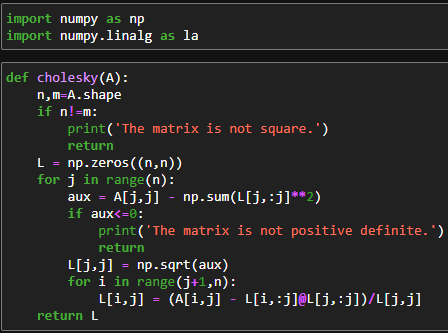
\includegraphics[scale=.8]{hw5 p1}
		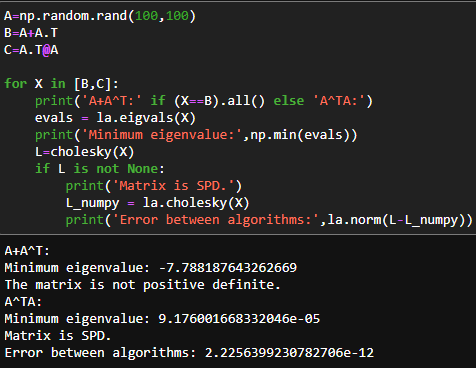
\includegraphics[scale=.7]{hw5 p2}
	\end{center}
	
	
	
\end{enumerate}
	
	
\end{document}